%\documentclass{UUThesisTemplate}
%\begin{document}
\chapter{Introduction}%
\epigraph{If a man will begin with certainties, he shall end in doubts; but\\ if he will be content to begin with doubts, he shall end in certainties.}{--- Francis Bacon}
%In this thesis we are interested in repetitions of words.  Indeed,
\noindent
Language is full of repetitions of words. %It is a statistical fact: we have a limited vocabulary and few words of our vocabulary are used frequently. %\citep{Zipf1936}. 
While reading this text, you have already encountered several of them without noticing it. And, in fact, it is normal; % to not pay attention to them:
 they are not an interesting event for our mind. 
However, sometimes we meet exceptions, %those exemptions are the object of this thesis. And some example of them are contained
% 
like
  in the following text:
\begin{quotation}
%``And as wondrous as it is, it cannot be reduced to a kind of simplification that we have often come to be admired. 
And yet, as wondrous as it is, our lives are complex. 
Our emotions are complex. 
Our intellectual desires are complex.  
%So I do believe that architecture as I see it needs to mirror that complexity in every single space that we have, in every intimacy that we possess. 

 When it comes to complexity there is no short term fix in a pill. % or anything else. 
%But
And your friends are long-term supports, and therefore, perhaps the most significant thing you can do to add more years to your life, and life to your years. %''
\end{quotation}

%You just came across some examples of rhetorical effects built with those uncommonly noticeable repetitions that create what we call \key{figures of speech}. 
\noindent
In this text, the repetition of the word ``complex'' three times, and the words ``life'' and ``years'' twice, probably caught your attention, or at least they caught your attention more than the repetition of the word ``as'' at the beginning of the text. %If you have to translate or read this text out loud, you will have to take into account this effect. We call such noticeable effect a figure of speech and when it involves a repetition we call it figure of repetition. 
We may not be conscious of making such a hierarchy in our attention to repetitions, but it is nevertheless an important part of our ability to correctly analyse, translate or read this text out loud in the most natural way. The authors of antiquity already knew about the properties of certain types of repetitions and included them in a subcategory of figures of speech which we call the figures of repetition. In this thesis we focus on three of them.
\bigskip

\noindent \key{Chiasmus},
%\footnote{The term comes Greek letter $\chi$ because of the cross this letter symbolises (see Figure~\ref{graphX} %======Schéma=======
%\begin{figure}[h!] 
%\begin{center}
%\includegraphics[scale=0.45]{images/X}
%\caption{Schema of a chiasmus.}
%\label{graphX}
%\end{center}
%\end{figure}
%%======Schéma=======).
%
%}
 which is the repetition of a pair of words in reverse order such as \Eref{ex:Mountain}.
%
\nnumsentence{If the \mn{mountain} won't come to \mn{Muhammad},\\ then \mn{Muhammad} must go to the \mn{mountain}. \label{ex:Mountain}}%
%

\noindent\key{Epanaphora}, the repetition of one or several words at the beginning of sentences as in \Eref{ex:Mylife}.%
%
\nnumsentence{\mn{My life is my} purpose.\\ 
\mn{My life is my} goal. \\
\mn{My life is my }inspiration. \label{ex:Mylife}}%
%
\noindent\key{Epiphora}, the repetition of one or several words at the end of the text, like in \Eref{ex:War}.
\nnumsentence{The United States, as the world knows, will never start \mn{a war}.\\
We do not want \mn{a war}.\\
We do not now expect \mn{a war}.\label{ex:War}}%
%
\vspace{-28pt}
\section{Research Questions and Contributions}

For a computer, locating all repetitions of words is trivial, but locating just those repetitions that achieve a rhetorical effect is not. Can this distinction be made automatically? The methods and models presented in this thesis focus on \textit{how} a computer can detect those figures of repetition. 
\begin{enumerate}
\item How should we define the task for detection of figures of repetition?
\item  What challenges are posed by different types of figures with respect to features and machine learning?

\item Can we automatically learn how to weight different features, and how much manually annotated data do we need for that?
\item How do we evaluate the performance on this task?
\item Which types of linguistic features are useful?
% \item To what extent can we distinguish rhetorical from accidental repetitions using automatically extracted linguistic features?
% \item Which types of linguistic features are useful?
% \item Can we automatically learn how to weight different features given the small amounts of annotated data?
%  \item  What challenges are posed by different types of figures with respect to features and machine learning?


\end{enumerate}
The main contributions of this thesis are:
\begin{enumerate}
\item A general model for detecting repetitive rhetorical figures, including a method of evaluation.
\item An experimental evaluation of this model with respect to chiasmus, epa\-naphora and epiphora, exploring the usefulness of different features and comparing machine learning and hand-tuning of feature weights.
\item A pilot study comparing the frequency of different figures in different text genres.
\item The development and testing of three systems of detection designed for the three repetitive figures we are looking for.
\item A number of corpora annotated for chiasmus, epanaphora and epiphora.
\end{enumerate}
\section{Outline of the Thesis}
%The outline of the thesis is as follow. 
%\bigskip

%\noindent Chapter 2 provides the motivation for studying the detection of repetitive figures. Through examples we will see that repetitive figures present a scientific interest from both a linguistic and computational linguistic point of view. We motivate the method used. Finally we explain why we focus on detection and not on generation.
%\bigskip

\noindent  Chapter 2 presents background information about figures of speech in general, and how they are split into categories. We describe the state of the art for their treatment in computational linguistics.
\bigskip

\noindent  Chapter  3 introduces the general method we use for all of our repetitive figure detectors. We will explain the model used for ranking, the evaluation method, the annotation process, and the tuning process. 
\bigskip

\noindent  Chapter 4 summarises the empirical results of our experiments. We analyse the performance of each system and discuss its statistical significance.
\bigskip


\noindent Chapter 5 summarises the contributions of the thesis. We conclude with a discussion of promising directions for future research.
\bigskip

\noindent  Chapter 6 provides a brief overview of the papers included in this thesis.

%\normalsize

%In Paper~\ref{pc} we show
%\includegraphics[scale=1]{X}
%\end{document}